%!TEX root = ../main.tex
\section{Goodcore Algorithm}
\label{sec:without}

In this section, we will  illustrate \ours algorithm in details for solving Eq.~\ref{eqa:expectation}, which is proven to be prohibitively expensive (Section~\ref{subsec:complexity}).  Then we focus on how to compute the expectation using possible worlds (Section~\ref{subsec:exp}) in the algorithm.

\subsection{Problem Complexity}~\label{subsec:complexity}

Let us first discuss the time complexity of  finding the optimum of Eq.~\ref{eqa:expectation}. 

\begin{theorem}
	\vspace{-0.3em} 
	The problem of expected optimal coreset selection over incomplete data is NP-hard. 
	\vspace{-0.6em} 
\end{theorem}

\begin{proof}
	Let us consider a special case that there is no missing value in $\train$. Our problem becomes the typical coreset selection problem over complete data, which has been proven to be NP-hard by reduction from the Minimum Vertex Cover problem~\cite{dinur2005hardness, mirzasoleiman2020coresets, DBLP:conf/icml/MirzasoleimanBL20}. Hence,  our problem is also NP-hard.
\end{proof}


\begin{theorem}
	\vspace{-0.3em}
	The problem of expected optimal coreset selection over incomplete data has the sub-modular property.
	\vspace{-0.3em}
\end{theorem}

\begin{proof}
	First, we regard $\mathrm{E}[C] = \sum_{k= 1}^{|\worlds|} p_kS_k$ as a utility function, where $S_k = \sum_{i=1}^n \min_{c_j\in C_k}\dist_{ij}$. In fact, $S_k$ can be regarded as a function of the coreset score computation over complete data, which has already  proven to have the sub-modular property~\cite{mirzasoleiman2020coresets, DBLP:conf/icml/MirzasoleimanBL20, killamsetty2021grad}. Therefore, consider the property that a non-negative linear combination of sub-modular functions is also sub-modular~\cite{lin2011class}. To be specific, given   any sub-modular function $g_1,g_2,\ldots,g_k$ and non-negative numbers $\alpha_1,\alpha_2,\ldots,\alpha_k$. Then the function $\mathcal{G}$ defined by $\mathcal{G}=\sum_{i=1}^k \alpha_i g_i$ is sub-modular.
    Hence, we can conclude that our studied problem is a sub-modular problem because $\mathrm{E}[C] = \sum_{k= 1}^{|\worlds|} p_kS_k$, where $p_k>0$.
    \vspace{-0.3em}
\end{proof}

\noindent \textbf{The greedy algorithm.} Given the sub-modular property, naturally, we can design a greedy algorithm with an approximate ratio. As shown in Algorithm~\ref{alg:framework}, we greedily add one tuple to the coreset at each iteration. The added tuple  should have the  largest utility computed by $\mathrm{E}[t|\core] = \mathrm{E}[\core] - \mathrm{E}[\core \cup \{t\}]$. Hence, the key component is that given the original train data $(\train)$ and a coreset ($\core$ or $\core \cup \{t\}$), how to compute the expectation of GA error ($\mathrm{E}[\core]$ or $\mathrm{E}[\core \cup \{t\}]$) of the coreset. However, it is non-trivial because of the large number of possible worlds.  We will first introduce how to compute the probability $p_k$, and describe the expectation computation in Section~\ref{subsec:exp}. After  $K$ tuples are added, we can impute missing tuples in the coreset generated by \ours.


\subsection{Expectation Computation}~\label{subsec:exp}

\noindent \textbf{Possible world probability.} To compute the expectation, it is inevitable to derive the probability of each possible world, which can be taken as a pre-processing step in our framework. 
To be specific, since tuples with missing values are always imputed independently~\cite{miao2022experimental}, given a possible world $\world_k$, the probability $p_k$ can be computed by $p_k = \prod\limits_{t\in \world_k, \mathbb{I}[t] = 1} p_k^t$, where $p_k^t$ denotes the probability of the appearance of tuple $t$ with $\mathbb{I}[t] = 1$. Besides, apparently  $p_k^t = 1$ when $\mathbb{I}[t] = 0$, so $p_k=1$ if there are only complete tuples.
Therefore, our focus is on how to get the value of  $p_k^t$, which can be solved by many approaches, like statistic methods and learning-based methods (see~\cite{miao2022experimental} for a survey). 
%
In this paper, we use the learning-based method~\cite{datawig} with a Python library~\cite{datawigpy} to generate the probability, which can be easily replaced by other libraries or domain-specific methods.
%
%\etitle{Statistic method.} A tuple $t$ may have multiple missing values in different attributes. The straightforward statistic method is to  obtain the probability distribution of values in each attribute through statistic information from $\train$. Afterwards, $p_k^t$ can be computed by simply multiplying the probabilities of these missing values.
%
%\etitle{Deep learning method.}
% Recently, more sophisticated deep learning based methods have been proposed for missing value imputation.
 During training, learning-based methods take $\train$ as input and learn a model $\mathcal{M}$ to describe the joint data distribution.
 For inference,  we have 
$ P(\attr_i | \mathbf{x}, v_{mask}) = \mathcal{M}(\mathbf{x}, v_{mask}, \omega^*)$, where the model takes as input the feature vector $\mathbf{x}$ of $t$, the mask vector $v_{mask}$ (indicating which attributes are missing) and the model parameter $\omega^*$, outputs the probability distribution of a missing attribute $\attr_i$.
 
Suppose that $t$ just  has one missing attribute  $\attr_i$, and then $v_{mask}$ is a one-hot vector with $v_{mask}[i] = 0$. Hence, we can directly obtain $p_k^t$  from the distribution $P(\attr_i | \mathbf{x}, v_{mask})$. For $t$ with multiple missing attributes, we can also compute $p_k^t$ using the chain rule. If $t$ has two missing values of $\attr_i$ and $\attr_j$, to compute $p_k^t$, we have to compute $P(\attr_i, \attr_j | \mathbf{x}, v_{mask})$, abbreviated as $P(\attr_i, \attr_j) = P(\attr_i)P(\attr_j | \attr_i)$. $P(\attr_i)$ can be obtained by masking the $i$-th and $j$-th attribute in $v_{mask}$.
 Then, we only mask the  $j$-th attribute  and impute different values of $\attr_i$ to obtain  $P(\attr_j | \attr_i)$.



 
 %For inference, given a tuple $t$, they leave missing attributes as masks and feed $t$ into the model. Then, the model can directly output the  distribution of missing values and we can obtain the value of  $p_k^t$. 

%\add{which takes an incomplete tuple $t$ along with a mask vector $v_{mask}$ as input and outputs the probability distribution of the missing values. Formally, we have }
%\begin{equation}\label{eq:probDL}
%	P(\attr_i | t, v_{mask}) = M_D(t, v_{mask}, \Omega^*)
%\end{equation}
%\add{where $\attr_i$ denotes the $i$-th attribute and $\Omega^*$ denotes the best parameters of $\mathcal{M}$.}

%\add{We now illustrate how to use $M_D$ to compute the probability of tuple $t$. If there is only one missing value in $t$, suppose $\attr_i$, we can derive the probability distribution using Eq.~\ref{eq:probDL}. We mask the $i$-th attribute (\ie $v_{mask}[i] = 0$) and feed $t$ along with $v_{mask}$ into $M_D$. $M_D$ outputs the probability of different values of $\attr_i$, \ie the probability distribution of $\attr_i$, denoted by $P(\attr_i)$. Apparently,  $P(t) = P(\attr_i)$.}

%\add{Consider that $t$ has two missing values $\attr_i$ and $\attr_j$. It is evident that the probability distribution of $t$ is the joint probability distribution of $\attr_i$ and $\attr_j$, \ie $P(t) = P(\attr_i, \attr_j)$. Then, we have $P(t) = P(\attr_i, \attr_j) = P(\attr_i)P(\attr_j | \attr_i)$. Following Eq.~\ref{eq:probDL}, we can first mask $\attr_i$, $\attr_j$ and obtain the probability distribution $P(\attr_i)$. Then, we only mask $\attr_j$ and impute different values of $\attr_i$ to obtain the marginal probability distribution $P(\attr_j | \attr_i)$. Finally, we multiple $P(\attr_i)$ and $P(\attr_j | \attr_i)$ to compute the probability of $t$. If $t$ has three or more missing values, we can use the chain rule to compute the probability. }



%\add{To be specific, suppose that we have a trained deep learning model $M_D$, which takes an incomplete tuple $t$ along with a mask vector $v_m$ as input and outputs the probability distribution of the missing values. For example, consider that we have a tuple $t$, $t[a] = \texttt{Null}$ and $t[b] = \texttt{Null}$. The range of $a$ and $b$ are $\{1,2\}$ and $\{F,M\}$, respectively. We first feed $t$ with masked attribute $a$ and $b$ into $M_D$. We can obtain the probability distribution of attribute $a$. Suppose that $p(t[a] = 1) = 0.6$ and $p(t[a] = 2) = 0.4$. Then, we can obtain two possible tuples $t[a = 1]$ and $t[a = 2]$. After feeding them into $M_D$, we can get the marginal probability distribution of attribute $b$. Suppose that $p(t[b] = F | t[a] = 1 ) = 0.5$, $p(t[b] = M | t[a] = 1) = 0.5$, $p(t[b] = F | t[a] = 2) = 0.8$ and $p(t[b] = M | t[a] = 2) = 0.2$. Then, we can get the probability distribution of tuple $t$ by multiple the marginal probability distribution of attribute $a$ and $b$, \ie $p(t[a] = 1, t[b] = F) = 0.3$, $p(t[a] = 1, t[b] = M) = 0.3$, $p(t[a] = 2, t[b] = F) = 0.32$ and $p(t[a] = 2, t[b] = M) = 0.08$. For the tuples with more two missing values, we can use the chain rule to solve this problem.}

\begin{example}
	In Figure~\ref{fig:missing}(a), suppose that for the first possible world, we have to compute $p_1 = p_1^2 \times  p_1^3 \times  p_1^4 \times  p_1^6$. For instance, to compute $p_1^3$, given the trained deep learning model, we feed 
	$\{\texttt{Lei}, \texttt{M}, \texttt{Mask}, \texttt{35}, \texttt{Mask}\}$ and a one-hot vector $\{1,1,0,1,0\}$  into the model and compute the probability distribution of this tuple, from which we can get $p_1^3$, \ie the probability of 	$\{\texttt{Lei}, \texttt{M}, \texttt{Sales}, \texttt{35}, \texttt{1}\}$.
	%which is the multiplication result of the probabilities of 
%	\vspace{-0.3em}
\end{example}


\begin{figure}[t]
 \centering
 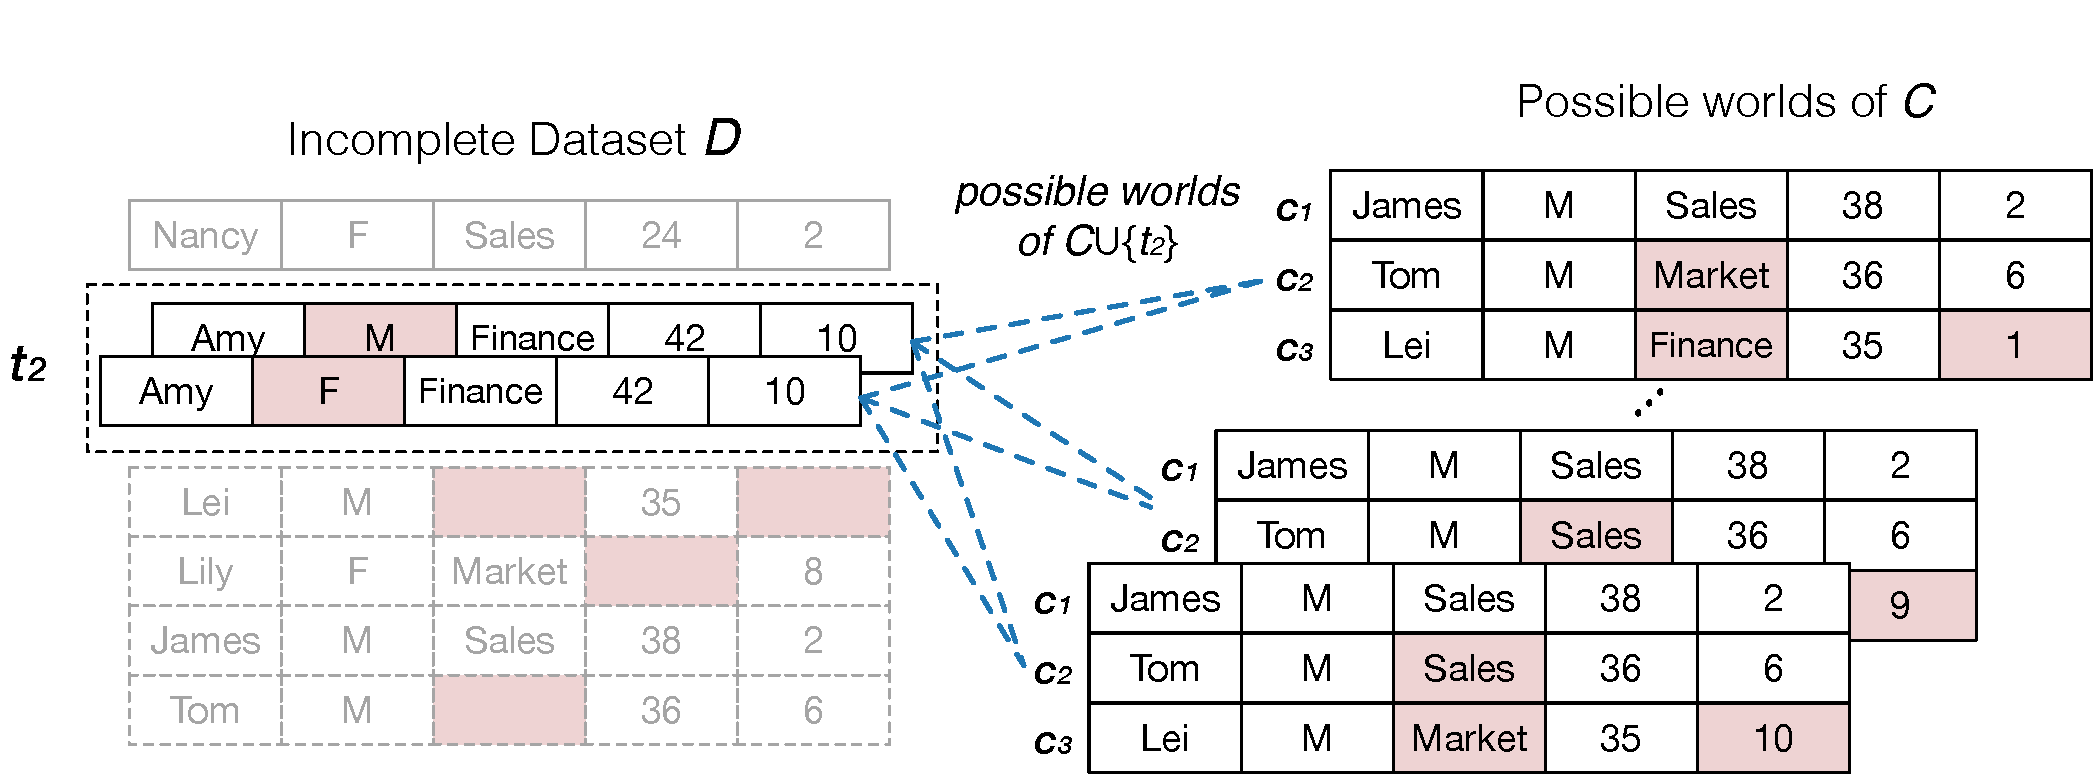
\includegraphics[width=0.6\textwidth]{figs/expectation}
% \vspace{-2.5em}
 \caption{Tuple-based expectation computation.}
 \label{fig:expectation}
% \vspace{-1.5em}
\end{figure}

Compared with statistical approaches, deep learning-based methods use more powerful models with good learning capacity and consider the correlation between attributes. For practitioners, they can use any ad-hoc method to compute the probability.



\stitle{Brute-force expectation computation.} Recap that $\mathrm{E}[C] = \sum_{k= 1}^{|\worlds|} p_k (\sum_{i=1}^n \min_{c_j\in C_k}\dist_{ij})$. Intuitively, the brute-force method is to enumerate each possible world, compute the probability and finally get the expectation. However, there are a huge number of possible worlds, which makes the  computation prohibitively expensive. Specifically, we assume the attribute number $M$ and $|\attr_m|, m\in [1, M]$ are  constants, so the number of possible worlds of each tuple is a constant, denoted by $L$.
Suppose that the number of tuples with missing values is $O(n)$, so the number of possible worlds ($|\worlds|$) is $O(L^n)$. Given a coreset $\core$, the time complexity to compute $\mathrm{E}[C]$ is $O(nL^n)$, which is rather expensive.

\stitle{Tuple-based expectation computation.} To further elaborate, we can easily expand $\mathrm{E}[C]$ as follows:


\begin{equation*}
\begin{aligned}
	\mathrm{E}[C] =& \uwave{p_1(\min_{c_j\in C_1}s_{1j}} + \min_{c_j\in C_1}s_{2j} + \cdots + \min_{c_j\in C_1}s_{nj})\\
	+ ~& \uwave{p_2(\min_{c_j\in C_2}s_{1j}} + \min_{c_j\in C_2}s_{2j} + \cdots + \min_{c_j\in C_2}s_{nj})+ \cdots \\
	+ ~& \uwave{p_{|\worlds|}(\min_{c_j\in C_{|\worlds|}}s_{1j}} + \min_{c_j\in C_{|\worlds|}}s_{2j} + \cdots + \min_{c_j\in C_{|\worlds|}}s_{nj}).
\end{aligned}
\end{equation*}

\noindent  We can see from the above equation that these underlined terms are only related to $t_1\in \train$ as well as  $\{\core_1, \core_2, \cdots, \core_{|\worlds|}\}$, \ie the coresets corresponding to the $|\worlds|$  possible worlds.
However, as the coreset $\core$ is much smaller than the full data $\train$, the number of possible worlds of $\core$ will be also much smaller than $|\worlds|$, and thus there will be many duplicates among $\{\core_1, \core_2, \cdots, \core_{|\worlds|}\}$.
Therefore, many of these underlined terms  have identical variable parts, \ie $\min_{c_j\in C_k} s_{1j}$, when they are associated with the same  $C_k$. These terms are \textit{like terms}. Combining these like terms  (\ie $\sum_{k=1}^{|\worlds|} p_k \min_{c_j\in C_k}s_{1j}$), we can get the expectation of $\min_{c_j\in C}s_{1j}$, denoted by $\mathrm{E}[\min_{c_j\in C}s_{1j}]$.




In short, we can convert the expectation computation over the possible worlds of the entire training set $\train$ to the sum of expectation of each tuple in $\train$, as follows:


\begin{equation}\label{eqa:tuple}
	\mathrm{E}[C] = \sum_{k= 1}^{|\worlds|} p_k (\sum_{i=1}^n \min_{c_j\in C_k}\dist_{ij})= \sum_{i=1}^n \mathrm{E}[\min_{c_j\in C}s_{ij}]
\end{equation}

\begin{example}
	Figure~\ref{fig:expectation} shows how to compute $\mathrm{E}[\min_{c_j\in C}s_{2j}]$. Instead of enumerating $|\worlds|$ possible worlds by the brute-force method, we can enumerate a much smaller number of possible worlds of $\core \cup t_2$, compute the corresponding probabilities and finally get the tuple expectation. Specifically, The left part of Figure~\ref{fig:expectation} shows the possible worlds of the tuple,  the right part shows the possible worlds of the coreset, and their combination is the possible worlds of $\core \cup t_2$. Then, following Eq.~\ref{eqa:tuple}, we can iterate the tuples in $\train$, compute their expectations and sum them up to derive $\mathrm{E}[C]$.
\end{example}




\iffalse
\vspace{-1em}
\begin{equation}\label{equation:triangle}
\begin{aligned}
&  \lVert\sum\limits_{i=1}^N \left( \df_i^+(\hypo) - \df_{\gamma(\map(i))}^+(\hypo) \right) \rVert 
\\
= &\lVert\sum_{i=1}^g  
\sum_{k\in G_i} \left(\df^+_k(\hypo) - \df^+_{\gamma(\map(k))}(\hypo) \right) \rVert 
\\
\le & \sum_{i=1}^g  \lVert
\sum_{k\in G_i}\left( \df^+_k(\hypo) - \df^+_{\gamma(\map(k))}(\hypo) \right) \rVert 
\\
\le & \sum_{i=1}^g  |G_i| \max_{k\in G_i}\lVert 
\df^+_k(\hypo) - \df^+_{\gamma(\map(k))}(\hypo)  \rVert \\
\end{aligned}
\end{equation}
\vspace{-.5em}
\fi

\stitle{Time complexity.} Since the coreset size is $K$, and  the number of tuples with missing values in the coreset is $O(K)$, the time complexity of computing $\mathrm{E}[C]$ using tuple-based method is $O(nL^K)$, where $K$ is much smaller than $n$, compared with the brute-force method. However, note that computing $\mathrm{E}[C]$ is just the third loop in the entire framework. Besides, the first two loops incrementally add $K$ tuples into the coreset, and sample $h$ tuples for tuple selection respectively. Hence, the overall time complexity of coreset selection over incomplete data is $O(KhnL^K)$, which is still expensive when $K$ is not small enough.  
In the next section, we involve the imputation-in-the-loop strategies to achieve further improvement.







